\documentclass[12pt]{exam}
\usepackage{amsthm}
\usepackage{bm}
\usepackage{libertine}
\usepackage[utf8]{inputenc}
\usepackage[margin=0.5in]{geometry}
\usepackage{amsmath,amssymb}
\usepackage{multicol}
\usepackage[shortlabels]{enumitem}
\usepackage{siunitx}
\usepackage{physics}
\usepackage{booktabs}
\usepackage{graphicx}
\usepackage{pgfplots}
\usepackage{listings}
\usepackage{tikz}
\bmdefine{\ii}{i}                       %% cuaternion i
\bmdefine{\jj}{j}                       %% cuaternion j
\bmdefine{\kk}{k}                       %% cuaternion k


\pgfplotsset{width=10cm,compat=1.9}
\usepgfplotslibrary{external}
\tikzexternalize

\newcommand{\class}{Math 261-001} % This is the name of the course 
\newcommand{\examnum}{Quiz 4} % This is the name of the assignment
\newcommand{\examdate}{September 26} % This is the due date





\begin{document}
\pagestyle{plain}
\thispagestyle{empty}

\noindent
\textbf{\class}\\
\textbf{\examnum}, \textbf{\examdate} \\

% Name \hfill CSU ID \# \hspace{2.25in}

%\vspace{10 pt}

\setlength{\tabcolsep}{3.5cm} % Default value: 6pt
\renewcommand{\arraystretch}{1.5}
\setlength\extrarowheight{1cm}
\begin{tabular}{ |c|c| } 
 \hline
 Name   & CSU ID \#  \\ 
 \hline
\end{tabular}
% ---
\vspace{10pt}

\textbf{Instructions.}  
This quiz has 4 multiple-choice questions. You must hand in at least 2, but you may choose 3 or all 4. Clearly circle the numbers of the questions you select. Space is provided to show work, correct work can earn partial credit even if the final answer is wrong. Each question is worth the same number of points, and your grade will be based on the average of the questions you hand in.



\iffalse

    \foreach \s in {1,...,5}{
          \choice $P_\s$ has no power 
     }%;
\fi


\begin{enumerate} 


\item Consider the expression
$$I=\int_{x=0}^{x=1}\int_{y=0}^{y=4}\sqrt{1+e^{2y}}\dd y\dd x+\int_{x=1}^{x=e^4}\int_{y=\log(x)}^{y=4}\sqrt{1+e^{2y}}\dd y\dd x$$
The region described by this integral is shaded in the following figure:
\begin{center}
    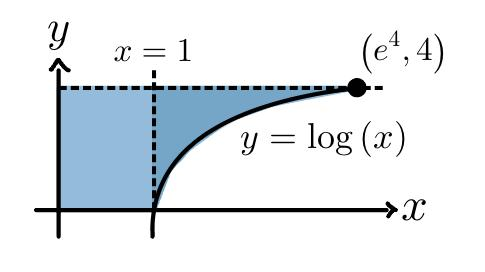
\includegraphics[width=0.4\textwidth]{fig2}
\end{center}
Rewriting in the order $\dd x \dd y$ it is possible to express $I$ as one integral:
$$\int_{\fbox{\hspace{2mm}\textbf{A}\hspace{2mm}}}^{\fbox{\hspace{2mm}\textbf{B}\hspace{2mm}}}\int_{\fbox{\hspace{2mm}\textbf{C}\hspace{2mm}}}^{\fbox{\hspace{2mm}\textbf{D}\hspace{2mm}}}\sqrt{1+e^{2y}}\dd x\dd y$$
Write the bounds of integration of the new integral in terms of $y$ and $x$ respectively, following the convention that $y=\cdots$ and $x=\cdots$\par
\begin{center}
    \textbf{A}:\fillin[$y=0$][1in], \textbf{B}:\fillin[$y=4$][1in], \textbf{C}:\fillin[$x=0$][1in], \textbf{D}:\fillin[$x=e^y$][1in].
\end{center}

\item Suppose $g$ is a differentiable function and consider the triple integral:
$$I=\int_{y=-1}^{y=1}\int_{x=0}^{x=\pi/2}\int_{z=0}^{z=\sqrt{\cos(x)}}zg'(y)\dd z\dd x\dd y.$$
When calculating the integral, we obtain the value
    \begin{checkboxes}
        \choice $I=0$
        \choice $I=1$
        \choice $I=2(g'(1)-g'(0))$
        \choice $I=\frac{g(1)-g(0)}{2}$
        \choice $I=g(1)-g(0)$
    \end{checkboxes}
\newpage

\item Let $T$ be the polyhedron with vertices $(0,1,0)$, $(1,1,0)$, $(1,1,1)$, $(0,1,1)$, and $(0,0,1)$.  
\begin{center}
    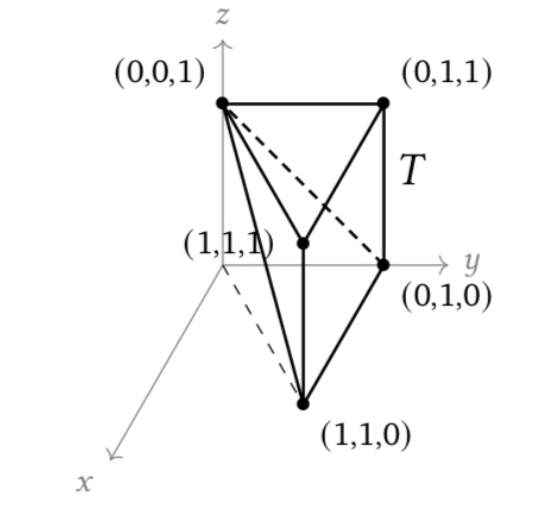
\includegraphics[width=0.4\textwidth]{fig1.png}
\end{center}
The volume of $T$ can be expressed by the following triple integral:
\begin{checkboxes}
    \choice $\displaystyle \int_0^1 \int_0^x \int_{1-x}^1 \dd z\dd y\dd x$
    \choice $\displaystyle \int_0^1 \int_{1-x}^1 \int_{1-x}^1 \dd z\dd y\dd x$
    \choice $\displaystyle \int_0^1 \int_{x}^1 \int_{1-y}^1 \dd z\dd y\dd x$
    \choice $\displaystyle \int_0^1 \int_{1-x}^1 \int_{1-y}^1 \dd z\dd y\dd x$
    \choice None of the above
\end{checkboxes}

\item Compute the value of the following double integral
$$I=\int_{\text{T}}e^{ax+by}\dd A,$$
where $T$ is the triangle bound by $x=0$, $y=0$ and $ax+by=1$.
\begin{checkboxes}
    \choice $I=1$
    \choice $I=a$
    \choice $I=b$
    \choice $I=ab$
    \choice $I=\frac{1}{ab}$
\end{checkboxes}
\end{enumerate}
\end{document}

